\newcommand{\psd}[1]{{\small\sffamily{\color{blue!60}#1}}}

In this tutorial we showcase the 2D bar problem simulation with one end
clamped wile being pulled at the other end. Body force is neglected and
the non clamped ends pull is approximated with Dirichlet displacement
\(u_1=1\). If this simulation is compared to the previous one from
tutorial 1 ans tutorial 2, the only difference now is that no body force
is applied and an additional Dirichlet condition is applied at the free
end of the bar. Here is how PSD simulation of this case can be
performed. he bar \(5\times1\) m\(^2\) in area is made up of material
with \(\rho=8\times 10^3\), \(E=200\times 10^9\), and \(\nu=0.3\).

\subsection{Step 1: Preprocessing}

First step in a PSD simulation is PSD preprocessing , at this step you
tell PSD what kind of physics, boundary conditions, approximations,
mesh, etc are you expecting to solve.

In the terminal \psd{cd} to the folder
\psd{/home/PSD-tutorials/linear-elasticity}. Launch
\psd{PSD\_PreProcess} from the terminal, to do so run the following
command.

\begin{lstlisting}[style=BashInputStyle]
PSD_PreProcess -problem linear_elasticity -dimension 2 -dirichletconditions 2 \
-postprocess u
\end{lstlisting}

After the \psd{PSD\_PreProcess} runs successfully you should see many
\psd{.edp} files in your current folder.

\textbf{What do the arguments mean ?}

\begin{itemize}
\item \psd{-problem linear\_elasticity} means that we are solving linear elasticity problem;
\item \psd{-dimension 2} means it is a 2D simulation;
\item \psd{-dirichletconditions 2} says we have two Dirichlet border;
\item \psd{-postprocess u} means we would like to have ParaView post processing files.

\end{itemize}

In comparison to preprocessing from other two tutorials (tutorial 1 and
2), notice that the body force flag \psd{-bodyforceconditions 1} is
missing. This is due to the fact that for this problem we assume null
body force. \psd{-dirichletconditions 2}, which notifies to PSD that
there are two Dirichlet borders in this simulation i) the clamped end
and ii) the pulled ends of the bar. To provide these Dirichlet
conditions of the two ends in \psd{ControlParameters.edp} set the
variables \psd{Dbc0On 2}, \psd{Dbc0Ux 0.}, and \psd{Dbc0Uy 0.}
signifying the clamped end (\(u_x=0,u_y=0\) on mesh label 2) and
\psd{Dbc1On 4}, \psd{Dbc1Ux 1.}, and \psd{Dbc1Uy 0.} signifying the
pulled end (\(u_x=1,u_y=0\) on label \psd{4}). Note that here at border
\psd{4} we have explicitly set \(u_2=0\) this means the bar is not
allowed to shrink (compress) in \(y\) direction, however you might wish
to allow the bar to compress. For such a simulation simply use
\psd{Dbc1On 4} and \psd{Dbc1Ux 1.}, and remove the term \psd{Dbc1Uy 0.}
therefor asking PSD not to apply constrain in \(y\) direction on the
pulled end.

Just like the previous tutorial the input properties \(E,\nu\) should be
mentioned in \psd{ControlParameters.edp}, use \psd{E = 200.e9}, and
\psd{nu = 0.3;}. The volumetric body force condition is mentioned in the
same file via variable \psd{Fbc0Fy -78480.0}, i.e
(\(\rho*g=8.e3*(-9.81)=-78480.0\)). One can also provide the mesh to be
used in \psd{ControlParameters.edp} , via
\psd{ThName = "../Meshes/2D/bar.msh"}
(\textit{note that mesh can also be provided in the next step}) .In
addition variable \psd{Fbc0On 1} has to be provided in order to indicate
the volume (region) for which the body force is acting, here \psd{1} is
the integer volume tag of the mesh.

\subsection{Step 2: Solving}

As PSD is a parallel solver, let us use 2 parallel processes to solve
this 2D bar case. To do so enter the following command:

\begin{lstlisting}[style=BashInputStyle]
PSD_Solve -np 2 Main.edp -mesh ./../Meshes/2D/bar.msh -v 0
\end{lstlisting}

Here \psd{-np 2} denote the argument used to enter the number of
parallel processes (MPI processes) used while solving.
\psd{-mesh ./../Meshes/2D/bar.msh} is used to provide the mesh file to
the solver. \psd{-v 0} denotes the verbosity level on screen.
\psd{PSD\_Solve} is a wrapper around \psd{FreeFem++} or
\psd{FreeFem++-mpi}. Note that if your problem is large use more cores.
PSD has been tested upto 13,000 parallel processes and problem sizes
with billions of unknowns, surely you will now need that many for the 2D
bar problem.

\subsection{Step 3: Postprocessing}

PSD allows postprocessing of results in ParaView. After the step 2
mentioned above finishes. Launch ParaView and have a look at the
\psd{.pvd} file in the \psd{VTUs\_DATE\_TIME} folder. Using ParaView for
postprocessing the results that are provided in the \psd{VTUs...}
folder, results such as those shown in
figure\textasciitilde{}\ref{bar-le-full-clamped} can be extracted.

\begin{figure}[h!]
\centering
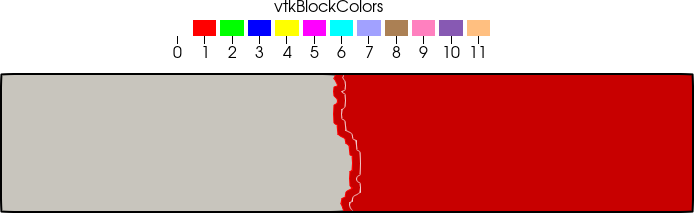
\includegraphics[width=0.39\textwidth]{./Images/le-2d-bar-clamped-pulled-partioned}\hfill
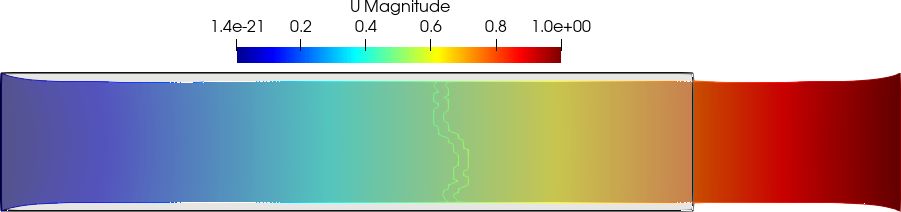
\includegraphics[width=0.5\textwidth]{./Images/le-2d-bar-clamped-pulled.png}
\caption{The 2D clamped bar problem: partitioned mesh and displacement field visualization in ParaView. \label{bar-le-full-clamped}}
\end{figure}

You are all done with your 2D linear-elasticity simulation.
